\documentclass{nsart_eng}
\usepackage{cite}
\usepackage{amsmath,amssymb}

% \usepackage{pscyr}
\usepackage[utf8]{inputenc}

\usepackage[russian]{babel}
\usepackage{graphicx}

\year{2016} \volume{0} \nomer{0} \firstpage{1}

\let\le\leqslant
\let\leq\leqslant
\let\ge\geqslant
\let\geq\geqslant

\newcommand{\hilb}[1]{\mathcal{H}_{#1}}
\newcommand{\cconj}[1]{\overline{#1}}
\newcommand{\hank}[1]{H_{#1}^{(1)}}

\newcommand{\mcF}{\mathcal{F}}
\newcommand{\mcH}{\mathcal{H}} % ???
\newcommand{\mcI}{\mathcal{I}}
\newcommand{\mcL}{\mathcal{L}} % L2 space
\newcommand{\mcO}{\mathcal{O}} % Big O
\newcommand{\mcP}{\mathcal{P}}


\newcommand{\bbC}{\mathbb{C}} % complex plane
\newcommand{\bbD}{\mathbb{D}} % complex unit disk
\newcommand{\bbH}{\mathbb{H}} % complex upper half-plane TODO add to template
\newcommand{\bbN}{\mathbb{N}}
\newcommand{\bbK}{\mathbb{K}}
\newcommand{\bbR}{\mathbb{R}}
\newcommand{\bbT}{\mathbb{T}} % complex unit circle
\newcommand{\bbZ}{\mathbb{Z}}

\newcommand{\eqdef}{\overset{\mathrm{def}}{=\joinrel=}}

\DeclareMathOperator{\dom}{dom}
\DeclareMathOperator{\ran}{Ran}
\DeclareMathOperator{\rng}{rng}

\newcommand{\todo}[1]{\textcolor{red}{{\large TODO: #1}}}

\newenvironment{elist}{\begin{easylist}[enumerate]}{\end{easylist}}
\newenvironment{ilist}{\begin{easylist}[itemize]}{\end{easylist}}

\newcommand{\myspecial}[1]{\mathrm{#1}}

% imaginary unit
\newcommand{\iu}{{i\mkern1mu}}


\newcommand{\ipcdot}{\ip{\cdot}{\cdot}}
\newcommand{\iip}[2]{[#1,#2]}
\newcommand{\iipcdot}{\iip{\cdot}{\cdot}}

\newcommand{\dsum}{\oplus}
\newcommand{\ddiff}{\ominus}
% indefinite direct sum
\newcommand{\idsum}{[+]}
\newcommand{\iddiff}{[-]}

\DeclarePairedDelimiter{\Vector}{\lparen}{\rparen}

\newcommand{\tit}{\textit}
\newcommand{\cls}{\overline}
\newcommand{\eps}{\varepsilon}


\newcommand{\argmin}{\operatornamewithlimits{argmin}}
\newcommand{\argmax}{\operatornamewithlimits{argmax}}

\renewcommand{\Re}{\operatorname{Re}}
\renewcommand{\Im}{\operatorname{Im}}
\renewcommand{\phi}{\varphi} % TODO is there a prettier way to do that

\newcommand{\eexp}[1]{e^{#1}}

\DeclareMathOperator\atanh{atanh}

% ???
% \newcommand{\abs}[1]{\left| #1 \right|}
% \newcommand{\norm}[1]{\left\lVert #1 \right\rVert}
\newcommand*\Eval[3]{\left.#1\right\rvert_{#2}^{#3}}
\usepackage{mathtools} % xmapsto, \Vector
\DeclarePairedDelimiter{\abs}{\lvert}{\rvert}
\newcommand{\eexp}[1]{e^{#1}}
\newcommand{\iu}{{i\mkern1mu}}


\begin{document}

\title[короткое название статьи]
{НАЗВАНИЕ СТАТЬИ}

\author[А.\,Б.~Иванов, C.\,C.~Claus, В.\,Г.~Петров]
{$^1$А.\,Б.~Иванов, $^{1}$C.\,C.~Claus, $^2$В.\,Г.~Петров}

\address{
$^1$ Санкт-Петербургский Национальный Исследовательский Университет Информационных Технологий, \\
Механики и Оптики,\\
Кронверкский пр., 49, Санкт-Петербург, 197101, Россия\\
$^2$ Swiss Federal University of Technology,\\
Sonneggstrasse, 5,  Zurich, CH-8092, Switzerland }

\email{ivanov@ivanov.ru, claus@claus.ch, petrov@petrov.ru }

УДК ???.??, ???.???.?% insert UDK

\begin{abstract}
Рассматривается задача рассеивания на квантовом графе $G$, представляющем из себя кольцо $\Omega$, связянное с каналом (TODO?) дельта-граничным условием???, параметризованным вещественной константой $a$. Изучается поведение системы при различных $a$, и полнота резонансных состояний графа $G$ в пространстве $\mcL_2(\Omega)$.
\end{abstract}

\keywords{задача рассеяния, квантовый граф, ???? TODO}

\maketitle

\section{Введение}

Текст введения

TODO
\[
\det S = 
\frac
{\cos\left(k\right) + {\left(\frac{a}{2 k} + i\right)} \sin\left(k\right) - 1}
{\cos\left(k\right) + {\left(\frac{a}{2 k} - i\right)} \sin\left(k\right) - 1}
\]


$a = 0$:

\[
\det S = \frac{\eexp{\iu k} - 1}{\eexp{-\iu k} - 1} = -\eexp{i k}
\]

% TODO \Im as Im??
\[
\ln \abs{\det S} = \ln \eexp{- \Im k} = -\Im k
\]

Преобразование Кэли: $\zeta = \frac{k - i}{k + i}$, обратное: $k = \iu \frac{1 + \zeta}{1 - \zeta}$.

Вычислим интеграл, сделаем это в пространстве единичного диска. $\Im k \to \Im \left( \iu \frac{1 + \zeta}{1 - \zeta} \right) $.

%  TODO вычислим интеграл под пределом в зависимости от R:
% TODO varphi??
\[
\lim \int\limits_{TODO ??? } \ln \abs{\det S(\zeta)} d \zeta = \lim \int\limits_{TODO ??? } \Im \left( \iu \frac{1 + \zeta}{1 - \zeta} \right)  d\zeta
\]

Перейдем в полярные координаты: $\zeta \to R \eexp{\iu \phi}, d\zeta \to R \iu \eexp{\iu \phi}$

% TODO proper d

Комплексный интеграл  $I$ складывается из сумм интегралов действительно части $I_R$ и мнимой $\iu I_I$. Рассчитаем мнимую часть подынтегрального выражения:

\begin{align*}
\Im \left(  \Im \left( \iu \frac{1 + R \eexp{\iu \phi}}{1 - R \eexp{\iu \phi}} \right) R \iu \eexp{\iu \phi} \right)
 &= R \Re \left(  \Re \left( \frac{1 + R \eexp{\iu \phi}}{1 - R \eexp{\iu \phi}} \right) \eexp{\iu \phi} \right) \\
 &= R \Re \left( \frac{1 + R \eexp{\iu \phi}}{1 - R \eexp{\iu \phi}} \right) \Re \left(   \eexp{\iu \phi} \right) \\
 &= R \Re \left( \frac{(1 + R \eexp{\iu \phi}) (1 - R \eexp{-\iu \phi}) }{(1 - R \eexp{\iu \phi}) (1 - R \eexp{-\iu \phi})} \right) \cos \phi \\
 &= R \Re \left( \frac{1 - R^2 + 2 \iu R \sin \phi}{1 + R^2 - 2 R \cos \phi} \right) \cos \phi \\
 &= R \frac{1 - R^2}{1 + R^2 - 2 R \cos \phi} \cos \phi \\
 % TODO calculate the integral properly
 &= 2 \pi R^2
\end{align*}

Можно видеть, что $\lim\limits_{R \to 1} I_I(R) = 2 \pi \ne 0$, следовательно, $S$ не является произведением Бляшке-Потапова, и, по критерию TODO как он называется?, система резонатных состояний графа $\Gamma$ не является полной на кольце $\Omega$.

% \[
% z \to R \eexp{\iu \phi}
% \]
% \[
% dz \to R \iu \eexp{\iu \phi} d \phi
% \]




\section{Название второго параграфа}
Текст

\section{Название третьего параграфа}

\subsection{Название подпараграфа 1}

Текст подпараграфа 1.

Ссылки на литературу в тексте делаются следующим образом
\cite{1,4}.

Формула в тексте: $c^2=a^2+b^2$.

Формула без нумерации:
$$
E=M \cdot C^2.
$$

Формула с нумерацией:
\begin{equation} \label{eq1}
\alpha (t) = \frac{ \beta (t)}{\gamma (t)}.
\end{equation}

Многострочные формулы можно задавать так:
\begin{multline} \label{eq2}
\sum\limits_{n=0}^\infty  {\frac{{f^{\left( n \right)} \left( {x_0 } \right)}}{{n!}}\left( {x - x_0 } \right)^n }  = \\
= f\left( {x_0 } \right) + \frac{{f'\left( {x_0 }
\right)}}{{1!}}\left( {x - x_0 } \right) +
 \frac{{f''\left( {x_0 } \right)}}{{2!}}\left( {x - x_0 } \right)^2 + \dots +
 \frac{{f^{\left( n \right)} \left( {x_0 } \right)}}{{n!}}\left( {x - x_0 } \right)^n  + \dots
\end{multline}

Ссылки на формулы задаются так  (\ref{eq1}).

Рисунок вставляется следующим образом:


\begin{figure}
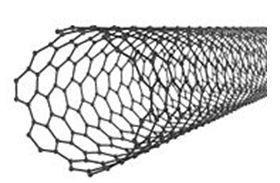
\includegraphics{fig1.png}
\caption{Черно-белая картинка}
\end{figure}




Таблица вставляется следующим образом:
\begin{table}[htbp]
\caption{Заголовок таблицы}
\begin{tabular}
{|c||c|c|c|} \hline Название 1 & Название 2 & Название 3 & Название 4\\
\hline \hline 1 & A & B & C \\ \hline 2 & $x_1$ & $y_1$ & $z_1$ \\
\hline 3 & $x_2$ & $y_2$ & $z_2$ \\ \hline
\end{tabular}
\end{table}

\subsection{Название подпараграфа 2}
Текст подпараграфа 2.

\section{Заключение}
Текст заключения

% \section*{Благодарности}
% Текст.

\begin{thebibliography}{99}
\bibitem{1}
Автор~А.\,А., Автор~Б.\,Б. {\it Название книги}.  Издательство,  город, 281~с. (2000)

\bibitem{2}
Автор~В.\,В., Автор~Г.\,Г. Название статьи. {\it Название журнала}, {\bf 1} (5), С 1 -- 3. (2000)

\bibitem{3}
Автор~Д.\,Д., Автор~Е.\,Е. Название доклада. Сборник трудов конференции "Конференция", место и дата, С. 47 -- 49

\bibitem{3}
Автор~Ж.\,Ж., Автор~З.\,З. Название статьи.  2010.
URL/arXiv: http://books.ifmo.ru/ntv.

\bibitem{4}
Название патента: патент 1111111 Россия MMM H04 B 1/36, Иванов И.И., владелец патента. OGOGO, N 2000131517/09, Bull. N 12, 3 с.


\end{thebibliography}

\end{document}
